\documentclass[tikz, border=10pt]{standalone}
\usepackage{amsmath}
\usepackage{tikz}
\usetikzlibrary{arrows.meta, positioning, fit, backgrounds, calc}

\definecolor{colInput}{RGB}{173,214,241}
\definecolor{colNorm} {RGB}{200,200,200}
\definecolor{colConv} {RGB}{130,179,220}
\definecolor{colPool} {RGB}{147,196,172}
\definecolor{colDense}{RGB}{253,192,134}
\definecolor{colOut}  {RGB}{240,240,240}

\tikzset{
  base/.style   = {draw, rounded corners=4pt, minimum width=72mm,
                   minimum height=8mm, font=\small, align=center, inner sep=4pt},
  input/.style  = {base, fill=colInput},
  norm/.style   = {base, fill=colNorm},
  conv/.style   = {base, fill=colConv},
  pool/.style   = {base, fill=colPool},
  concat/.style = {base, fill=colPool!60},
  dense/.style  = {base, fill=colDense},
  outbox/.style = {base, fill=colOut},
  arr/.style    = {-{Stealth[length=5pt]}, thick},
}

\begin{document}
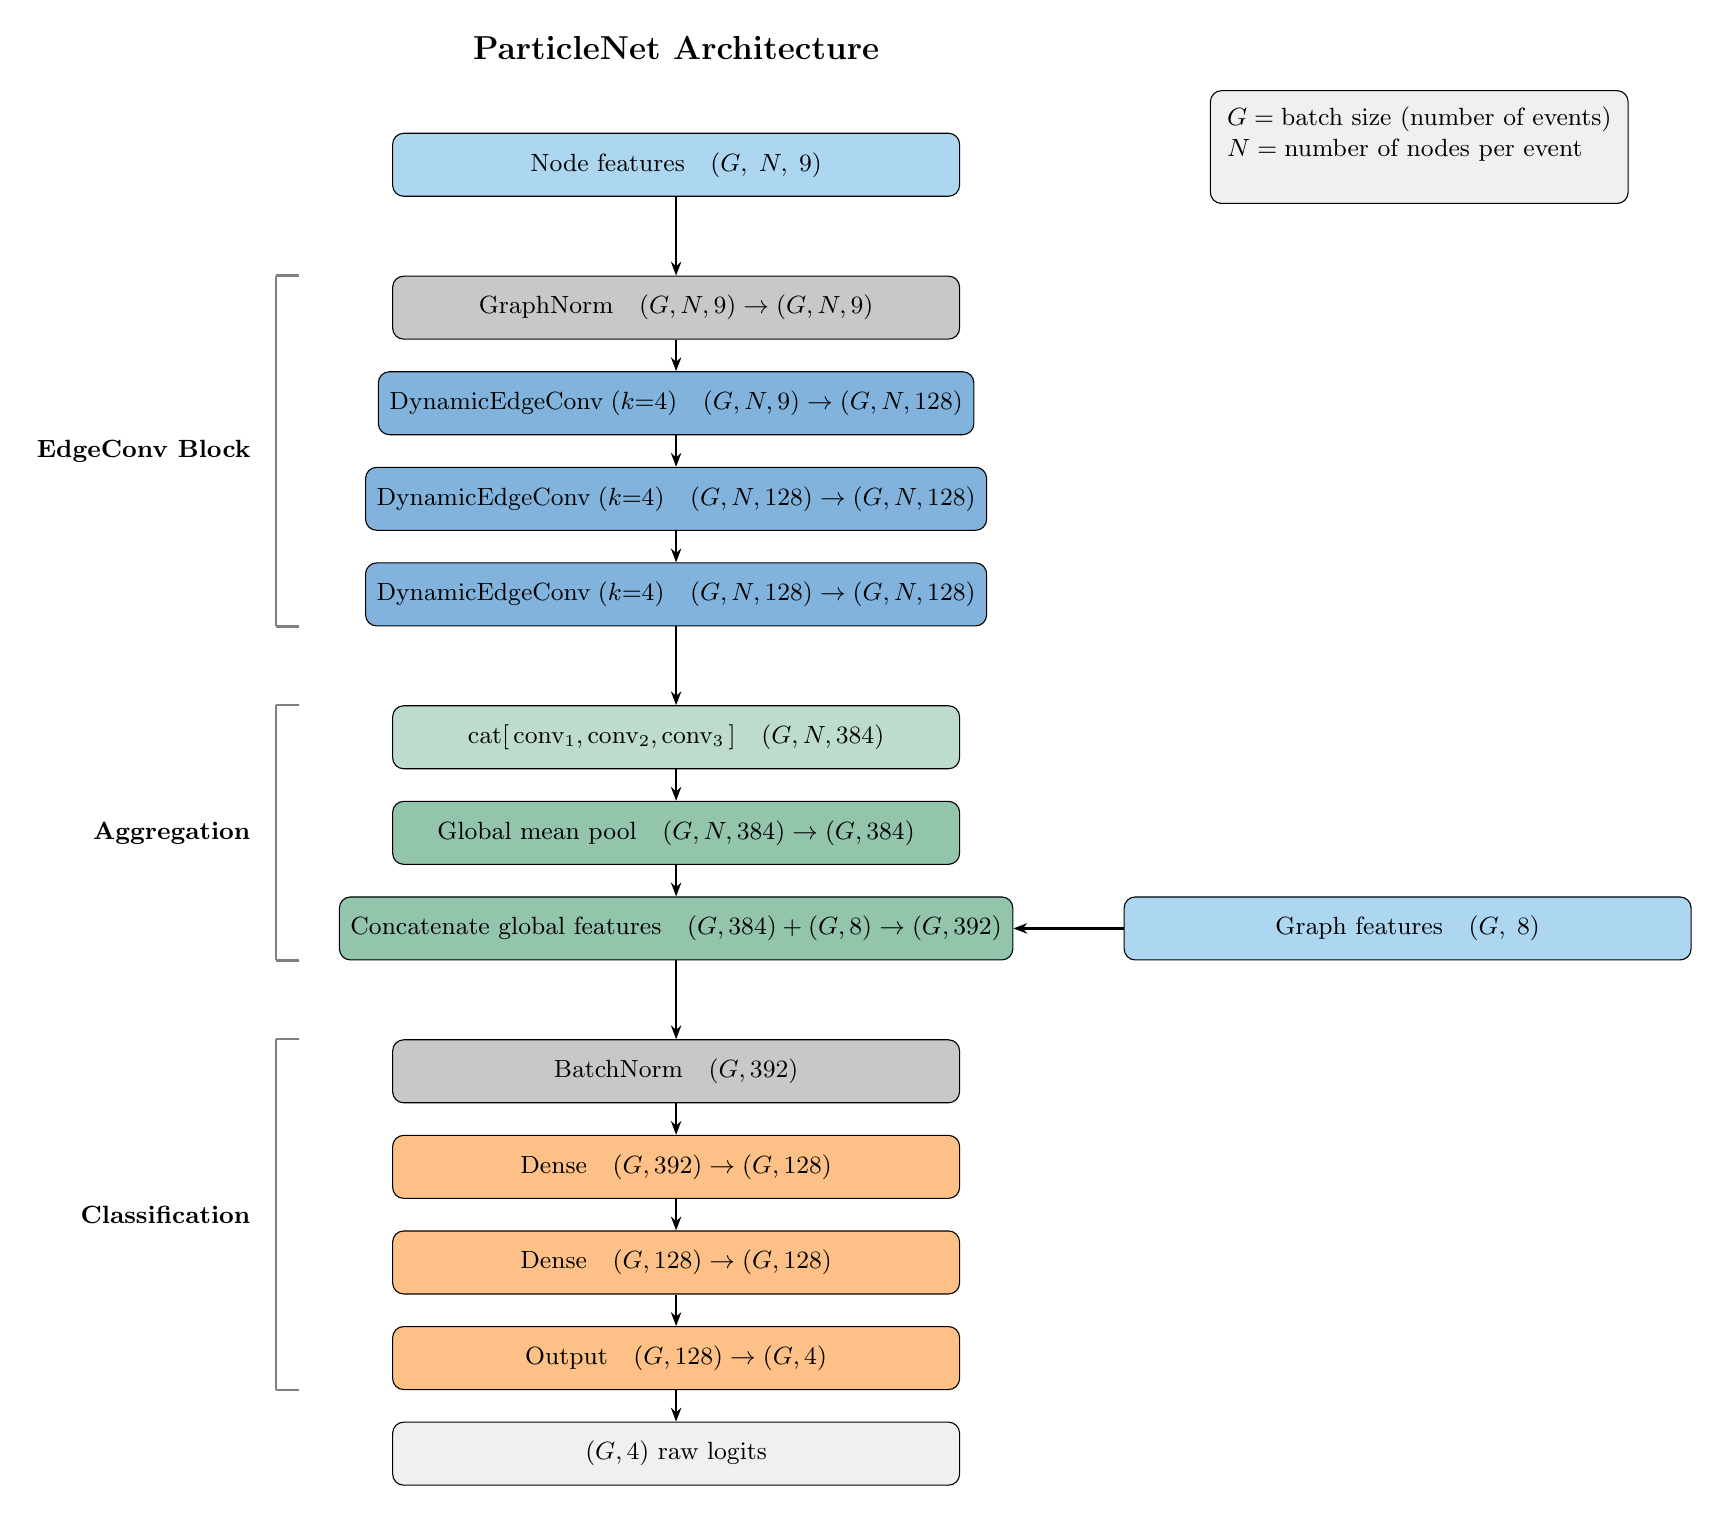
\begin{tikzpicture}[node distance=5mm]

%% ── title ───────────────────────────────────────────────────────────────────
\node[font=\large\bfseries] (title) {ParticleNet Architecture};

%% ── Input ────────────────────────────────────────────────────────────────────
\node[input, below=8mm of title] (nodeIn)
  {Node features\quad$(G,\;N,\;9)$};

%% ── EdgeConv Block ───────────────────────────────────────────────────────────
\node[norm,  below=10mm of nodeIn] (gn)
  {GraphNorm\quad$(G,N,9)\to(G,N,9)$};
\node[conv,  below=4mm of gn]  (c1)
  {DynamicEdgeConv\;($k{=}4$)\quad$(G,N,9)\to(G,N,128)$};
\node[conv,  below=4mm of c1]  (c2)
  {DynamicEdgeConv\;($k{=}4$)\quad$(G,N,128)\to(G,N,128)$};
\node[conv,  below=4mm of c2]  (c3)
  {DynamicEdgeConv\;($k{=}4$)\quad$(G,N,128)\to(G,N,128)$};

%% ── Aggregation ──────────────────────────────────────────────────────────────
\node[concat, below=10mm of c3] (cat)
  {cat$[\,$conv$_1$,\,conv$_2$,\,conv$_3$$\,]$\quad$(G,N,384)$};
\node[pool,   below=4mm of cat] (gmp)
  {Global mean pool\quad$(G,N,384)\to(G,384)$};
\node[pool,   below=4mm of gmp] (catG)
  {Concatenate global features\quad$(G,384)+(G,8)\to(G,392)$};

% Graph features input: right of catG
\node[input, right=14mm of catG] (graphIn)
  {Graph features\quad$(G,\;8)$};

%% ── Classification ───────────────────────────────────────────────────────────
\node[norm,  below=10mm of catG] (bn0)
  {BatchNorm\quad$(G,392)$};
\node[dense, below=4mm of bn0]  (d1)
  {Dense\quad$(G,392)\to(G,128)$};
\node[dense, below=4mm of d1]   (d2)
  {Dense\quad$(G,128)\to(G,128)$};
\node[dense, below=4mm of d2]   (out)
  {Output\quad$(G,128)\to(G,4)$};

\node[outbox, below=4mm of out] (label)
  {$(G,4)$ raw logits};

%% ── arrows ───────────────────────────────────────────────────────────────────
\draw[arr] (nodeIn) -- (gn);
\draw[arr] (gn)  -- (c1);
\draw[arr] (c1)  -- (c2);
\draw[arr] (c2)  -- (c3);
\draw[arr] (c3)  -- (cat);
\draw[arr] (cat) -- (gmp);
\draw[arr] (gmp) -- (catG);
\draw[arr] (catG)-- (bn0);
\draw[arr] (bn0) -- (d1);
\draw[arr] (d1)  -- (d2);
\draw[arr] (d2)  -- (out);
\draw[arr] (out) -- (label);
\draw[arr] (graphIn.west) -- (catG.east);

%% ── [ brackets ───────────────────────────────────────────────────────────────
%% All brackets share the same x, derived after all nodes are placed.
%% We use the west side of the widest node (catG) minus a fixed offset.

% EdgeConv Block
\draw[thick, gray]
  (gn.north  west -| catG.west) +(-8mm, 0) coordinate (E1T)
  (c3.south  west -| catG.west) +(-8mm, 0) coordinate (E1B);
\draw[thick, gray]
  (E1T) -- (E1B)
  (E1T) -- ++(3mm, 0)
  (E1B) -- ++(3mm, 0);
\node[font=\small\bfseries, anchor=east] at ($(E1T)!0.5!(E1B) + (-2mm,0)$)
  {EdgeConv Block};

% Aggregation
\draw[thick, gray]
  (cat.north  west -| catG.west) +(-8mm, 0) coordinate (E2T)
  (catG.south west -| catG.west) +(-8mm, 0) coordinate (E2B);
\draw[thick, gray]
  (E2T) -- (E2B)
  (E2T) -- ++(3mm, 0)
  (E2B) -- ++(3mm, 0);
\node[font=\small\bfseries, anchor=east] at ($(E2T)!0.5!(E2B) + (-2mm,0)$)
  {Aggregation};

% Classification
\draw[thick, gray]
  (bn0.north west -| catG.west) +(-8mm, 0) coordinate (E3T)
  (out.south  west -| catG.west) +(-8mm, 0) coordinate (E3B);
\draw[thick, gray]
  (E3T) -- (E3B)
  (E3T) -- ++(3mm, 0)
  (E3B) -- ++(3mm, 0);
\node[font=\small\bfseries, anchor=east] at ($(E3T)!0.5!(E3B) + (-2mm,0)$)
  {Classification};

%% ── legend (upper right corner) ─────────────────────────────────────────────
\node[draw, rounded corners=4pt, fill=colOut, font=\small, align=left,
      inner sep=6pt, anchor=north east] (legend)
  at ([xshift=-8mm, yshift=-8mm]title.north east -| graphIn.east) {%
  $G$\;=\;batch size (number of events)\\
  $N$\;=\;number of nodes per event\\
};

\end{tikzpicture}
\end{document}
